\chapter{Grammatiche}
  Come visto in precedenza, spesso gli automi vengono utilizzati come modelli per il riconoscimento di linguaggi. Gli automi sono quindi uno strumento formale per la descrizione e la definizione di un determinato linguaggio, costituito dall'insieme delle stringhe accettate dall'automa stesso.

  Un altro formalismo utilizzato per la definizione di linguaggio sono le cosiddette grammatiche formali, che definiscono un linguaggio fornendo il procedimento mediante cui si ottengono le stringhe appartenenti al linguaggio stesso. 
  
  \section{Introduzione}

  Una grammatica formale è un insieme di regole per costruire stringhe appartenenti ad un determinato linguaggio, attraverso il meccanismo di riscrittura, che consiste in un insieme di tecniche che determinano come sostituire le parti di una formula con parti più semplificate. In generale, un meccanismo di riscrittura consiste in un insieme di regole linguistiche, di cui una descrive l'oggetto principale come una sequenza di componenti. Ogni componente si può raffinare da elementi via via sempre più dettagliati, fino ad ottenere una sequenza di componenti elementari.

  Una grammatica non è altro che un meccanismo linguistico, composto dall'oggetto principale, detto anche simbolo iniziale, da un insieme di componenti, a loro volta da sostituire durante il processo di derivazione, detti anche simboli non terminaliun insieme di elementi di base, detti anche simboli elementari, e da un insieme di regole di raffinamento o sostituzioni, chiamate produzioni.

  \begin{definition} \label{definizione grammatica}
    Una grammatica G è una tupla di 4 elementi \(G = <V_T, V_N, P, S>\), dove:
    \begin{itemize}
      \item \(V_T\) è un insieme di simboli terminali (solitamente indicati con lettere minuscole), detto anche alfabeto terminale;
      \item \(V_N\) è un insieme di simboli non terminali (solitamente indicati con lettere maiuscole), tali che \(V_T \cap V_N = \emptyset\), detto anche alfabeto non terminale; V indica \(V_T\cup V_N\);
      \item P è un insieme finito di \(V_N^+\times V^*\), detto anche insieme delle produzioni di G. Un elemento \(p=<\alpha, \beta> \in P\) si indica con \(\alpha\to\beta\), in cui \(\alpha\) è la parte sinistra di p, mentre \(\beta\) è la parte destra di p;
      \item S è un elemento particolare di \(V_N\), detto assioma o simbolo iniziale. 
    \end{itemize}
  \end{definition}

  Quindi, un elemento che deve essere ancora raffinato è un simbolo non terminale, un elemento di base è un simbolo terminale, le componenti di un oggetto possono essere sia simboli terminali che non terminali, mentre una produzione corrisponde ad una regola di raffinamento.

  \begin{definition}
    Data una grammatica G, si definisce su \(V^*\) la relazione binaria di derivazione immediata, indicata con il simbolo \(\Rightarrow\) da \(\alpha\) a \(\beta\). Tale relazione sussiste se e solo se \(\alpha=\alpha_1\gamma\alpha_2, \beta=\alpha_1\delta\alpha_2\), con \(\alpha_1, \alpha_2, \delta \in V^*, \gamma \in V_N^+, \gamma\to\delta\in P\).
  \end{definition}

  Data la definizione di derivazione immediata, si può anche definire la chiusura riflessiva e transitiva, indicata con il simbolo \(\Rightarrow^*\), che opera su una serie di stringhe (di simboli elementari o non elementari), anzichè che su una sola stringa.

  Date le precedenti definizioni, si può ora definire il linguaggio generato da una grammatica, tramite la seguente definizione:
  \begin{definition}
    Data una grammatica G, il linguaggio L(G) generato da G è definito come:

    \(L(G)=\{x\;|\;S\Rightarrow^*x, x\in V_T^*\}\)
  \end{definition}

  Quindi il linguaggio generato da una grammatica è costituito da tutte e sole le stringhe di simboli terminali, derivati a partire dall'assioma \(S\), applicando un numero qualsiasi di sostituzioni.

  \section{Classificazione}
  Una volta definite cosa siano le grammatiche, è possibile classificarle in base alle loro proprietà e in base alla forma ammessa per le produzioni. Tale classificazione viene anche detta Gerarchia di Chomsky, tramite cui si dividono le grammatiche in quattro categorie:
  \begin{itemize}
    \item Grammatiche di tipo 0 (non ristrette): sono grammatiche definite come nella \ref{definizione grammatica}, ovvero grammatiche che non possiedono nessuna restrizione nel tipo di produzione;
    \item Grammatiche di tipo 1 (sensibili al contesto): sono grammatiche a cui si introduce il vincolo per cui le produzioni possono essere solo nella forma \(\alpha A\beta\to\alpha\gamma\beta\), dove \(\alpha, \beta, \gamma\in V\) e \(A\in V_N\), con \(\gamma\neq\varepsilon\); inoltre, la derivazione \(S\to\varepsilon\) è consentita solo se \(S\) non appare a destra in nessuna regola di derivazione;
    \item Grammatiche di tipo 2 (non contestuali): sono grammatiche a cui si introduce il vincolo per cui ad ogni produzione \(\alpha\to\beta \in P\) si verifica che \(\;|\;\alpha\;|\; =1\) (quindi \(\alpha \in V_N\)) e \(\beta\in V^*\);
    \item Grammatiche di tipo 3 (regolari): sono grammatiche a cui si introduce il vincolo per cui ad ogni produzione \(\alpha\to\beta \in P\) si verifica che \(\;|\;\alpha\;|\; = 1\) (quindi \(\alpha \in V_N\)) e che \(\beta\) sia in una sola delle seguenti forme: \(aB\), \(Ba\), \(a\) oppure \(\varepsilon\), con \(a\in V_T\) e \(B\in V_N\); inoltre, la derivazione \(S\to\varepsilon\) è consentita solo se \(S\) non appare a destra in nessuna regola di derivazione;
  \end{itemize} 

  \begin{figure}[!h]
    \begin{center}    
      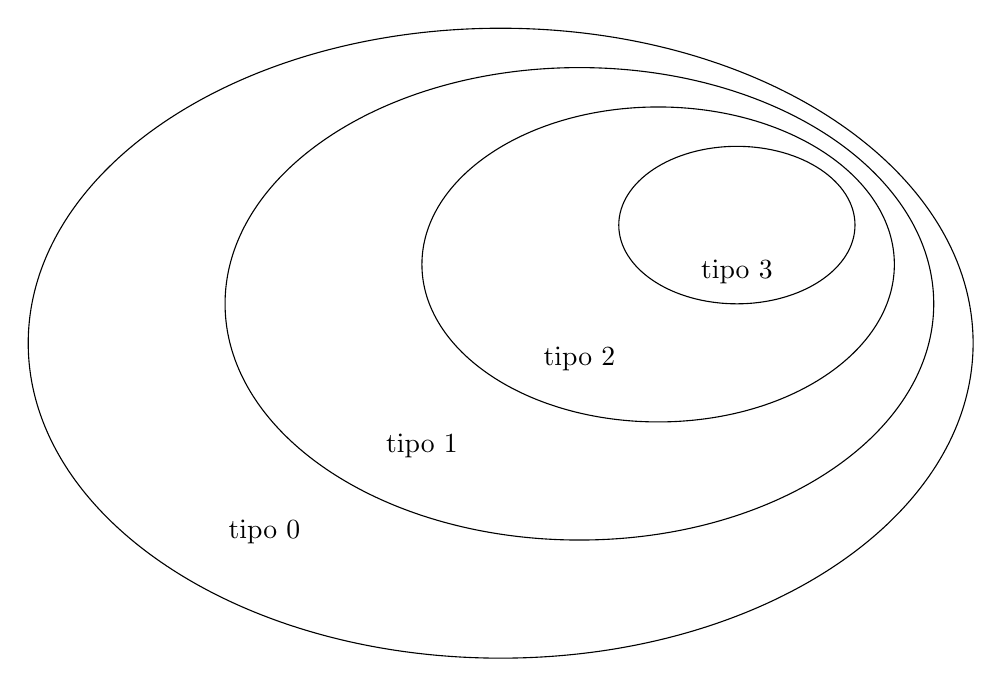
\begin{tikzpicture}
        \foreach \X [count=\Y starting from 0.75] 
        in {tipo 3, tipo 2, tipo 1, tipo 0} {
          \draw (-\Y,-\Y/2) circle ({1.5*\Y} and \Y);
          \node at (1-2*\Y,-1.1*\Y) {\X}; 
        }
      \end{tikzpicture}
    \end{center}
    \caption{Gerarchia di Chomsky}    
  \end{figure}

  \section{Grammatiche e Automi}
  Studiando le grammatiche e i linguaggi da esse generate, si può osservare una certa corrispondenza con gli automi analizzati nei capitoli precedenti. Si introducono qui alcuni teoremi che mettono in luce la correlazione esistente fra automi e grammatiche.

  \begin{theorem}
    Dato un FSA A, è possibile costruire una grammatica regolare (di tipo 3) G ad esso equivalente, ossia in grado di riconoscere lo stesso linguaggio riconosciuto da A, e viceversa. Dunque, le grammatiche regolari e gli automi a stati finiti sono modelli differenti per descrivere la stessa classe di linguaggi. 
  \end{theorem}
  Dato un FSA \(A=<I, \delta, q_0, F>\), si può costruire una grammatica \(G=<V_N,V_T, P, S>\) regolare, tale che:
  \begin{itemize}
    \item \(V_N=Q\);
    \item \(V_T=I\);
    \item \(S=q_0\);
    \item \(\forall B\to bC\iff C\in\delta(B,b)\);
    \item \(\forall B\to\varepsilon, B\in F\)
  \end{itemize}
  Data una grammatica \(G=<V_N, V_T, P, S>\) regolare, si può costruire un FSA \(A=<I, \delta, q_0, F>\), tale che:
  \begin{itemize}
    \item \(Q=V_N\cup\{q_F\}\);
    \item \(I=V_T\);
    \item \(q_0=S\);
    \item \(F=\{q_F\}\)
    \item \(\forall A\to bC, C\in \delta(A,B)\);
    \item \(\forall A\to b, q_F\in\delta(A,b)\)
  \end{itemize}

  In generale, l'automa a stati finiti \(A\), ottenuto a partire dalla grammatica regolare \(G\), è non deterministico.

  \begin{theorem}
    Dato un NPDA A è possibile costruire una grammatica G non contestuale (di tipo 2) ad esso equivalente, ossia in grado di riconoscere lo stesso linguaggio riconosciuto da A, e viceversa. Dunque, le grammatiche non contestuali e gli automi a pila non deterministici sono modelli differenti per descrivere la stessa classe di linguaggi.
  \end{theorem}

  \begin{theorem}
    Data una TM M utilizzata come accettatore di linguaggi è possibile costruire una grammatica generale G (di tipo 0) ad essa equivalente, ossia in grado di riconoscere lo stesso linguaggio riconosciuto da M, e viceversa.Dunque, le grammatiche non ristrette e le macchine di Turing sono modelli differenti per descrivere la stessa classe di linguaggi.
  \end{theorem}

  \section{Espressioni Regolari}
  Un'espressione regolare è un'espressione utilizzabile per denotare un linguaggio attraverso la struttura delle stringhe che lo compongono.

  \begin{definition}
    Dato un alfabeto di simboli terminali denotato con \(V_T\), si definiscono su di esso le espressioni regolari e i corrispondenti linguaggi denotati:
    \begin{itemize}
      \item \(\emptyset\) è un'espressione regolare che denota il linguaggio vuoto;
      \item \(\forall a\in V_T, a\) è un'espressione regolare che denota il linguaggio formato solo dal simbolo \(a\);
      \item Se \(R_1\) ed \(R_2\) sono espressioni regolari, anche la loro unione, indicata con \(R_1+R_2\) o \(R_1\;|\;R_2\), è un'espressione regolare;
      \item Se \(R_1\) ed \(R_2\) sono espressioni regolari, anche la loro concatenazione, indicata con \(R_1\cdot R_2\), è un'espressione regolare;
      \item Se R è un'espressione regolare, anche la stella di Kleene di R, indicata con \(R^*\), è un'espressione regolare.
    \end{itemize}
  \end{definition}

  Nessun'altra stringa è un'espressione regolare.

  Gli operatori \(\;|\;, \cdot, ^*\) definiti per le espressioni regolari, hanno un implicito ordine di applicazione, se non indicato diversamente dall'uso delle parentesi. In particolare, * ha la precedenza rispetto a \(\cdot\), che ha a sua volta la precedenza su \(\;|\;\).
  
  Inoltre, vale anche il seguente teorema:
  \begin{theorem}
    La classe dei linguaggi denotati dalle espressioni regolari coincide con la classe dei linguaggi regolari. 
  \end{theorem}

  \section{Riepilogo}

  \begin{table}[ht]
    \caption{Relazione fra grammatiche, linguaggi e automi}
    \centering
    \vspace{10px}
    \begin{tabular}{c c c c}
      Gerarchia & Grammatiche & Linguaggi & Automa minimo \\ 
      \hline
      tipo 0 & Generali & Ricorsivamente enumerabili & TM\\
      tipo 1 & Dipendenti dal contesto & Dipendenti dal contesto & LBA*\\
      tipo 2 & Non contestuali & Non contestuali & NPDA\\
      tipo 3 & Regolari & Regolari & FSA\\
    \end{tabular}
  \end{table}

  * Gli LBA (Linear Bounded Automata) sono un particolare tipo di macchina di Turing non deterministica in cui la lunghezza del nastro è dunzione lineare della dimensione della stringa in ingresso. Tali automi non sono stati trattati in questo documento. 